\section{Arquitectura de Software}
Algunos errores comunes en la definición de la arquitectura de sistemas de software es considerarla como una tarea reservada solo para los lideres técnicos,
que se busca promover una visión acotada a solo la vista tecnológica, que se tiene una ausencia de vínculos estrechos con el problema de negocio a resolver, o que es la ubicación de recursos tecnológicos sin justificación

Por esto, se acordó que era necesario una visión mas rica, aparece Zachman para hacer una definición de la arquitectura que tuviese parte de lo mencionado. El resultado fue una matriz que plantea diferentes preguntas y cuestiones.

\begin{figure}[!htb]
    \centering
    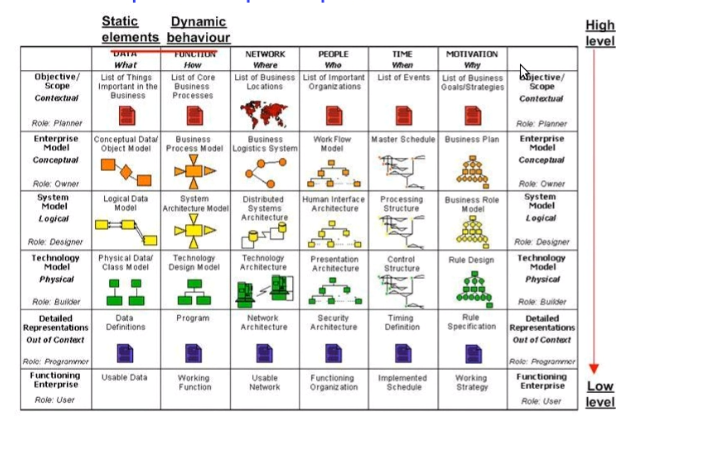
\includegraphics[width=0.8\textwidth]{img/matriz.PNG}
\end{figure}

Esto se usa para ver las diferentes cuestiones, y ayudar a documentar lo que queremos realizar. Deja al costado la visión tecnológica, y abarca el problema de una forma mas
general.

En el siguiente diagrama se pueden ver las componentes que representan a una arquitectura.

\begin{figure}[!htb]
    \centering
    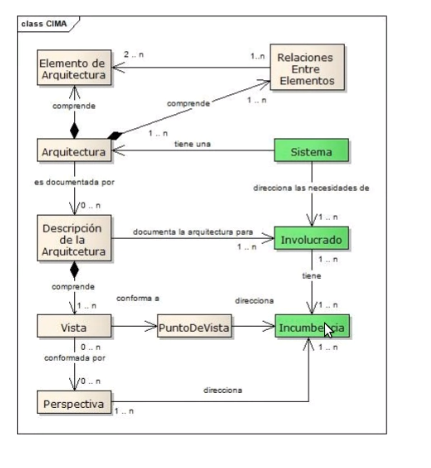
\includegraphics[width=0.6\textwidth]{img/componentes de arquitectura.PNG}
\end{figure}


\newpage
\subsection*{Puntos de vista}
Es un conjunto de patrones, plantillas y convenciones para la construcción de un tipo de vista. Se definen incumbencias. Se reflejan en ellas las directrices, principios y modelos para la construcción de sus vistas.

\begin{figure}[!htb]
    \centering
    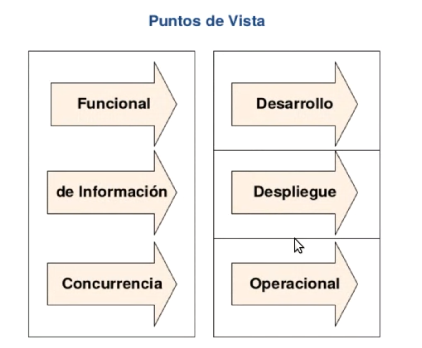
\includegraphics[width=0.7\textwidth]{img/vistas.PNG}
\end{figure}


\subsubsection*{Funcional}
Describe las funcionalidades que ofrece el sistema, sus responsabilidades, interfaces e interacciones primarias. Tiene un impacto significativo en el sistema.

\subsubsection*{Información}
Describe la forma en que la arquitectura almacena, manipula, maneja, y distribuye información. Esta ligada directamente a los datos.

\subsubsection*{Desarrollo}
Describe la arquitectura que soporta el proceso de desarrollo de software, el ámbito donde se va a realizar. Comunica los aspectos de la arquitectura de interés
para los actores involucrados en la construcción, pruebas, mantenimiento y la mejora del sistema.

\subsubsection*{Concurrencia}
Describe la estructura de la concurrencia del sistema y mapea elementos
funcionales a las unidades de concurrencia para identificar claramente las
partes del sistema que pueden ejecutarse al mismo tiempo y cómo esto se
coordina y controla

\subsubsection*{Despliegue}
Describe el ambiente en el que el sistema se implementará, incluyendo la
captura de las dependencias que el sistema tiene en su ambiente de tiempo
de ejecución.

Se ocupa de las cuestiones de instalar lo realizado en el ambiente productivo. Dependencias de archivos, bases de datos, etc.

\subsubsection*{Operacional}
Describe cómo el sistema será operado, administrado, y soportado cuando
se esté ejecutando en su entorno de producción. 

\subsection*{Perspectivas}
Son los requerimientos no funcionales, cuestiones vinculadas a la seguridad, performance, disponibilidad, regulaciones (legal), accesibilidad, tiempos de respuesta, etc
Queremos trasladarlos a nuestra arquitectura. 

\begin{figure}[!htb]
    \centering
    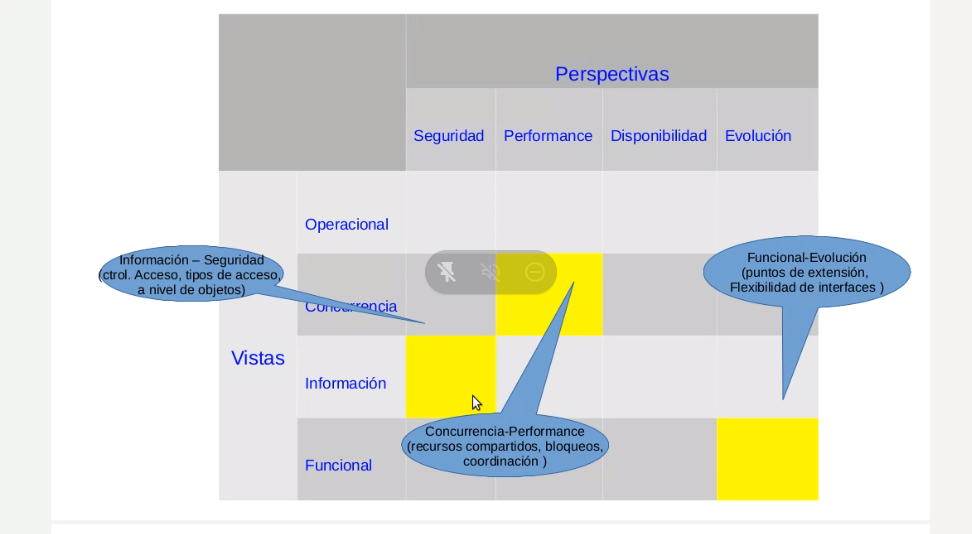
\includegraphics[width=0.7\textwidth]{img/ejemplo hipotetico vista perspectiva.PNG}
\end{figure}

\begin{figure}[!htb]
    \centering
    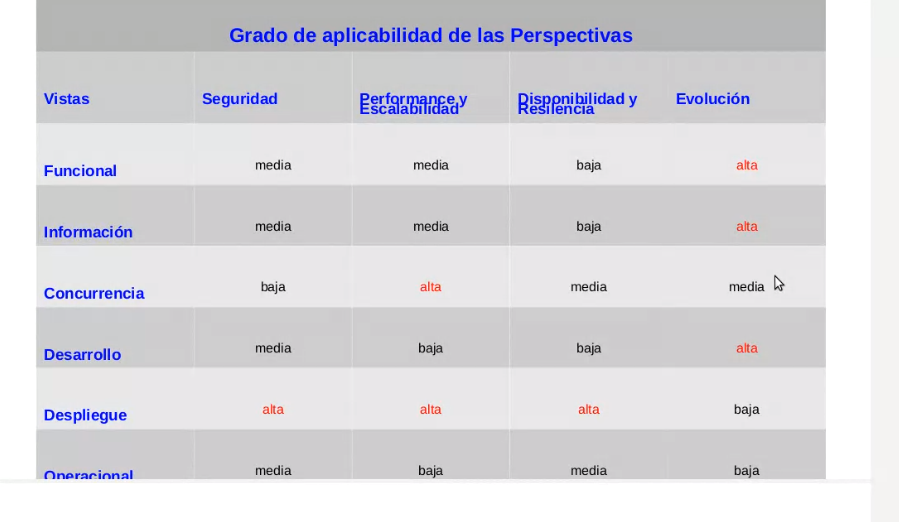
\includegraphics[width=0.8\textwidth]{img/matriz vistas ej.PNG}
\end{figure}

\newpage
\subsection*{Beneficios}

\begin{itemize}
\item Proporciona una partición de la arquitectura en un conjunto de modelos relacionados.
\item Provee un punto de vista para cada tipo de involucrado.
\item Ayuda a evaluar las propiedades o atributos de calidad asociados a las necesidades de cada involucrado y con la relevancia acorde en cada vista.
\item Provee un marco sistemático para la definición de la arquitectura
\end{itemize}


\subsection*{Definición de la arquitectura}

\begin{enumerate}
\item Guías, usamos la matriz de Zachman
\item Resultados, son los que obtenemos de las respuestas, tienen que proporcionar claridad a los requerimientos. Permiten evaluar las 
\item Contexto
\item Actividades de Soporte
\item Actividades de Definición
\item Relación con la metodología de desarrollo
\end{enumerate}


\begin{figure}[!htb]
    \centering
    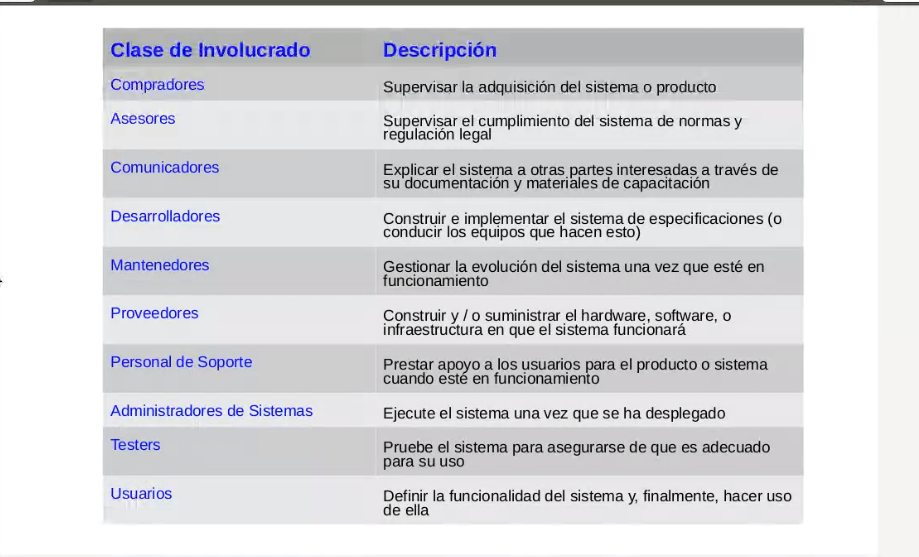
\includegraphics[width=0.7\textwidth]{img/ejemplos de involucrados.PNG}
    \caption{Ejemplos de involucrados}
\end{figure}


\subsubsection*{Escenarios}
\begin{itemize}
\item Un ejemplo de escenario seria sacar cable de red, cambian las reglas, nos obligan a plantearnos que pasa en este caso.
\end{itemize}


\subsubsection*{Validación de la arquitectura}
\begin{itemize}
\item Es necesario para validar abstracciones, comprobar que es correcta en lo técnico, generar confianza, explicar aspectos no claros.
\end{itemize}


\subsubsection*{Criterio terminación}
\begin{itemize}
\item Cuando la revisión con todos los involucrados no genera comentarios, observaciones o propuestas de cambio.
\item Cuando usted como arquitecto revisor de su arquitectura no tiene observaciones ni propuestas de cambio
\item Cuando se haya generado una descripción de la arquitectura que comunique y clarifique las expectativas e incumbencias de todos los involucrados.
\end{itemize}


% parcial desarrollo modelo dominio, defs arquitectura, criterios de diseño vinculado al problema